%%%%%%%%%%%%%%%%%%%%%%%%%%%%%%%%%%%%%%%%%%%%%%%%%%%%%%%%%%%%%%%%%%%%%%%%%%%%%%%%
%% Plantilla de memoria en LaTeX para TFG/TFM - Universidad Rey Juan Carlos
%%
%% Por Gregorio Robles <grex arroba gsyc.urjc.es>
%%     Felipe Ortega   <felipe.ortega@urjc.es>
%%     Grupo de Sistemas y Comunicaciones (GSyC)
%%     Escuela Técnica Superior de Ingenieros de Telecomunicación
%%     Universidad Rey Juan Carlos
%%
%% (Muchas ideas tomadas de Internet, colegas del GSyC, antiguos alumnos...
%%  etc. Muchas gracias a todos)
%%
%% La última versión de esta plantilla está siempre disponible en:
%%     https://github.com/glimmerphoenix/plantilla-memoria
%%
%% - Ejecución en sistema local:
%% Para obtener el documento en PDF, ejecuta en la shell:
%%   make
%%
%% A diferencia de la anterior versión, que usaba la herramienta pdfLaTeX 
%% para compilar el documento, esta nueva versión de la plantilla usa
%% XeLaTeX. Es un compilador más moderno que, entre otras mejoras, incluye
%% soporte nativo para caracteres con codificación UTF-8, traducción políglota
%% de referencias (usando Biblatex) y soporte para fuentes OTF. Esta última
%% característic permite, por ejemplo, insertar iconos de la colección 
%% Fontawesome en el texto.
%%
%% XeLaTeX viene ya incluido en todas las distribuciones modernas de LaTeX.
%%
%% - Edición y ejecución en línea: 
%% Puedes descargar y subir la plantilla a
%% Overleaf, un editor de LaTeX colaborativo en línea. Overleaf ya tiene
%% instalados todos los paquetes LaTeX y otras dependencias software para
%% que esta plantilla compile correctamente.
%%
%% IMPORTANTE: Si compilas este documento en Overleaf, recuerda cambiar
%% la configuración (botón "Menu" en la esquina superior izquierda de la interfaz)
%% y elegir la opción Compiler --> XeLaTeX. En caso contrario no funcionará.
%%
%% - Nota: las imágenes deben ir en PNG, JPG, EPS o PDF. También se pueden usar
%% imágenes en otros formatos con algunos cambios en el preámbulo del documento.

%%%%%%%%%%%%%%%%%%%%%%%%%%%%%%%%%%%%%%%%%%%%%%%%%%%%%%%%%%%%%%%%%%%%%%%%%%%%%%%%

\documentclass[a4paper, 12pt]{book}

%%-- Geometría principal (dejar activada la siguiente línea en la versión final)
\usepackage[a4paper, left=2.5cm, right=2.5cm, top=3cm, bottom=3cm]{geometry}
%%-- Activar esta línea y comentar la anterior en modo borrador, para comentarios al margen
%\usepackage[a4paper, left=2.5cm, right=2.5cm, top=3cm, bottom=3cm, marginparwidth=60pt]{geometry}

%%-- Hay que cargarlo antes que las traducciones
\usepackage{listing}                    % Listados de código

% Traducciones en XeLaTeX
\usepackage{polyglossia}
\setmainlanguage{spanish}    % Comenta esta línea si tu memoria es en inglés

% Traducciones particulares para español
% Caption tablas
\gappto\captionsspanish{
	\def\tablename{Tabla}
	\def\listingscaption{Código}
	\def\refname{Bibliografía}
	\def\appendixname{Apéndice}
	\def\listtablename{Índice de tablas}
	\def\listingname{Código}
	\def\listlistingname{Índice de fragmentos de código}
}

%% Tipografía y estilos
\usepackage[OT1]{fontenc}               % Keeps eulervm happy about accents encoding

% Símbolos y fuentes matemáticas elegantes: Euler virtual math fonts
% ¡Importante! Carga siempre las fuentes math AMS Euler ANTES QUE fontspec
\usepackage{amsmath}
\usepackage{amssymb}
\usepackage[OT1,euler-digits,euler-hat-accent,small]{eulervm}

% En XeLaTeX las fuentes se especifican con fontspec
\usepackage{fontspec}
\defaultfontfeatures{Scale=MatchLowercase, Ligatures=TeX}     % Default option in font config

% Fix para fuentes usadas con operadores y \mathrm
\DeclareSymbolFont{operators}{\encodingdefault}{\familydefault}{m}{n}

% Configura la fuente principal (serif): MinionPro
\setmainfont[Scale=0.96]{TeX Gyre Pagella}
% Configura la fuente sans-serif (\sffamily)
\setsansfont[Scale=MatchLowercase]{Lato}
% Configura la fuente para letra monoespaciada: Source Code Pro, escala 0.85
\setmonofont[Scale=0.85]{Source Code Pro}

%%-- Familias de fuentes específicas
%%-- Se pueden definir etiquetas para familias de fuentes personalizadas
%%-- que luego puedes emplear para cambiar el formato de una parte de texto
%%-- Ejemplo:
% \newfontfamily{\myriadprocond}{Myriad Pro Semibold Condensed.otf}

%%-- Opciones de interlineado y espacios
\linespread{1.07}                   % Aumentar interlineado para fuentes tipo Palatino
\setlength{\parskip}{\baselineskip} % Separar párrafos con línea en blanco

%%-- Hipervínculos
\usepackage{url}

%%-- Gráficos y tablas
\PassOptionsToPackage{
    dvipdfmx,usenames,dvipsnames,
    x11names,table}{xcolor}             % Definiciones de colores
\PassOptionsToPackage{xetex}{graphicx}

\usepackage{subfig}                     % Subfiguras
\usepackage{pgf}
\usepackage{svg}                        % Integración de imágenes en formato SVG
\usepackage{float}                      % H para posicionar figuras
\usepackage{booktabs}                   % Already loads package xcolor
\usepackage{multicol}                   % multiple column layout facilities
\usepackage{colortbl}                   % For coloured tables
\usepackage{comment}

%%-- Bibliografía con Biblatex y Biber
% Más info:
% https://www.overleaf.com/learn/latex/Biblatex_bibliography_styles
% https://www.overleaf.com/learn/latex/biblatex_citation_styles
\usepackage[
    backend=biber,
    style=numeric,
    sorting=nty
    ]{biblatex}
\addbibresource{memoria.bib}
\DeclareFieldFormat{url}{\mkbibacro{URL}\addcolon\nobreakspace\url{#1}}
%\usepackage[nottoc, notlot, notlof, notindex]{tocbibind} %% Opciones de índice

%%-- Matemáticas e ingeniería
% El paquete units permite mostrar unidades correctamente
% Permite escribir unidades con espaciado y estilo de fuente correctos
\usepackage[ugly]{units}         
% Ejemplo de uso: $\unit[100]{m}$ or $\unitfrac[100]{m}{s}$
% Entornos matemáticos
\newtheorem{theorem}{Theorem}

% Paquetes adicionales
\usepackage{url}                        %% Gestión correcta de enlaces
\usepackage{float}                      %% H para posicionar figuras
\usepackage[nottoc, notlot, notlof, notindex]{tocbibind}    %% Opciones de índice
\usepackage{metalogo}                   %% Múltiples logos para XeLaTeX

% Fuentes especiales y glifos
\usepackage{ccicons}                % Creative Commons icons
\usepackage{metalogo}               % XeTeX logo
\usepackage{fontawesome5}           % Fontawesome 5 icons
\usepackage{adforn} 

% Blindtext
% Opciones pangram, bible, random (defecto)
\usepackage[pangram]{blindtext}
% Lorem ipsum
\usepackage{lipsum}
% Kant lipsum
\usepackage{kantlipsum}

\usepackage{fancyvrb}               % Entornos verbatim extendidos
	\fvset{fontsize=\normalsize}    % Tamaño de fuente por defecto en fancy-verbatim
	
% Configura listas (itemize, enumerate) con iconos personalizados
% Fácil reinicio de numeración con enumerate
% Info: http://ctan.org/pkg/enumitem
\usepackage[shortlabels]{enumitem}
% Usar \usageitem para configurar iconos personalizados en listas
\newcommand{\usageitem}[1]{%
	\item[%
	{\makebox[2em]{\strut\color{GSyCblue} #1}}%
	]
}

%%-- Definición de colores personalizados
% \definecolor{LightGrey}{HTML}{EEEEEE}
% \definecolor{darkred}{rgb}{0.5,0,0}     %% Refs. cruzadas
% \definecolor{darkgreen}{rgb}{0,0.5,0}   %% Citas bibliográficas
% \definecolor{darkblue}{rgb}{0,0,0.5}    %% Hiperenlaces ordinarios (también ToC)

%%-- Configuración fragmentos de código
%%-- Minted necesita Python Pygments instalado en el sistema para funcionar
%%-- En Overleaf ya está instalada esta dependencia
% \usepackage[center, labelfont=bf]{caption}
\usepackage{minted}

%%-- Se debe cargar aquí para evitar warnings
\usepackage{csquotes}                   % Para traducciones con biblatex

%%-- Glosario de términos
\usepackage[acronym]{glossaries}
\makeglossaries
\loadglsentries{glossary}

% % Definición de cabeceras del documento, usando fancyhdr
% \usepackage{fancyhdr}
% %% Configuración de cabeceras para el cuerpo principal del documento
% \pagestyle{fancy}
% \fancyhead{}
% \fancyhead[RO,LE]{\myriadprocond{\thepage}}
% \renewcommand{\chaptermark}[1]{\markboth{\chaptername\ \thechapter.\ #1}{}}
% \renewcommand{\sectionmark}[1]{\markright{\thesection.\ #1}}
% \fancyhead[RE]{\myriadprocond{\leftmark}}
% \fancyhead[LO]{\myriadprocond{\rightmark}}
% \renewcommand{\headrulewidth}{0pt}
% \setlength{\headheight}{15pt} %% Al menos 15pt para evitar warning al compilar
% \fancyfoot{}
% %% Configuración para páginas con cabecera en blanco
% \fancypagestyle{plain}{%
% \fancyhf{}% clear all header and footer fields
% \fancyhead[RO,LE]{\myriadprocond{\thepage}}
% \renewcommand{\headrulewidth}{0pt}%
% \renewcommand{\footrulewidth}{0pt}%
% }

%%-- Metadatos del doc
\title{Memoria del Proyecto}
\author{Nombre del autor}

%%-- Hiperenlaces, siempre se carga al final del preámbulo
\usepackage[colorlinks]{hyperref}
\hypersetup{
    pdftoolbar=true,	% Muestra barra de herramientas en Adobe Acrobat
	pdfmenubar=true,	% Muestra menú en Adobe Acrobat
	pdftitle={Título doc en ventana del visor o navegador},
	pdfauthor={Nuria Díaz Jérica},
	pdfcreator={ETSII/ETSIT, URJC},
	pdfproducer={XeLaTeX},
	pdfsubject={Topic1, Topic2, Topic3},
	pdfnewwindow=true,              %links open in new window
    colorlinks=true,                % false: boxed links; true: coloured links
    linkcolor=Firebrick4,           % enlaces internos 
    citecolor=Aquamarine4,          % enlaces a citas bibliográficas
    urlcolor=RoyalBlue3,            % hiperenlances ordinarios
    linktocpage=true                % Enlaces en núm. pág. en ToC
}

%%%---------------------------------------------------------------------------
% Comentarios en línea de revisión
% Este bloque se puede borrar cuando finalizamos el borrador

% \usepackage[colorinlistoftodos]{todonotes}
% \usepackage{verbatim}
%%%---------------------------------------------------------------------------

\begin{document}

%%-- Configuración común para todos los entornos listing
%%-- Descomentar para usar y personalizar valores
%\lstset{%
%breakatwhitespace=true,
% breaklines=true, 
% basicstyle=\footnotesize\ttfamily,
% keywordstyle=\color{blue},
% commentstyle=\color{green!40!black}, 
% language=Python} 
 

%%%%%%%%%%%%%%%%%%%%%%%%%%%%%%%%%%%%%%%%%%%%%%%%%%%%%%%%%%%%%%%%%%%%%%%%%%%%%%%%
% PORTADA

\begin{titlepage}
\begin{center}
\begin{tabular}[c]{c c}
%
\includegraphics[bb=0 0 194 352, scale=0.25]{logo} &
\includegraphics[scale=1.5]{img/LogoURJC.png}
%&
%\begin{tabular}[b]{l}
%\Huge
%\textsf{UNIVERSIDAD} \\
%\Huge
%\textsf{REY JUAN CARLOS} \\
%\end{tabular}
\\
\end{tabular}

\vspace{3cm}

\Large 
INGENIERÍA DE ROBÓTICA SOFTWARE

\vspace{0.4cm}

\large
Curso Académico 2021/2022

\vspace{0.8cm}

Trabajo Fin de Grado

\vspace{2cm}

\LARGE UN TÍTULO DE PROYECTO LARGO\\
EN DOS LÍNEAS
\vspace{3cm}

\large
Autor/a : Nuria Díaz Jérica \\
Tutor/a : Dr. Nombre del Profesor/a
\end{center}
\end{titlepage}

\newpage
\mbox{}
\thispagestyle{empty} % para que no se numere esta pagina


%%%%%%%%%%%%%%%%%%%%%%%%%%%%%%%%%%%%%%%%%%%%%%%%%%%%%%%%%%%%%%%%%%%%%%%%%%%%%%%%
%%%% Para firmar
\clearpage
\pagenumbering{gobble}
\chapter*{}

\vspace{-4cm}
\begin{center}
\LARGE
\textbf{Trabajo Fin de Grado/Máster}

\vspace{1cm}
\large
Entrenamiento y Aplicación de Modelos de Aprendizaje Automático en Dispositivos con Capacidad de Cómputo Limitada\\
Título del Trabajo con Letras Capitales para Sustantivos y Adjetivos

\vspace{1cm}
\large
\textbf{Autor/a :} Nuria Díaz Jérica  \\
\textbf{Tutor/a :} Dr. Nombre del profesor/a

\end{center}

\vspace{1cm}
La defensa del presente Proyecto Fin de Grado/Máster se realizó el día 3\qquad$\;\,$ de
\qquad\qquad\qquad\qquad \newline de 20XX, siendo calificada por el siguiente tribunal:


\vspace{0.5cm}
\textbf{Presidente:}

\vspace{0.8cm}
\textbf{Secretario:}

\vspace{0.8cm}
\textbf{Vocal:}


\vspace{0.8cm}
y habiendo obtenido la siguiente calificación:

\vspace{0.8cm}
\textbf{Calificación:}


\vspace{0.8cm}
\begin{flushright}
Móstoles/Fuenlabrada, a \qquad$\;\,$ de \qquad\qquad\qquad\qquad de 20XX
\end{flushright}

%%%%%%%%%%%%%%%%%%%%%%%%%%%%%%%%%%%%%%%%%%%%%%%%%%%%%%%%%%%%%%%%%%%%%%%%%%%%%%%%
%%%% Dedicatoria

\chapter*{}
%\pagenumbering{Roman} % para comenzar la numeración de paginas en numeros romanos
\begin{flushright}
\textit{Aquí normalmente \\
se inserta una dedicatoria corta \\}
\end{flushright}

%%%%%%%%%%%%%%%%%%%%%%%%%%%%%%%%%%%%%%%%%%%%%%%%%%%%%%%%%%%%%%%%%%%%%%%%%%%%%%%%
%%%% Agradecimientos

\chapter*{Agradecimientos}
%\addcontentsline{toc}{chapter}{Agradecimientos} % si queremos que aparezca en el índice
\markboth{AGRADECIMIENTOS}{AGRADECIMIENTOS} % encabezado 

Aquí vienen los agradecimientos\ldots

Hay más espacio para explayarse y explicar a quién agradeces su apoyo o ayuda para
haber acabado el proyecto: familia, pareja, amigos, compañeros de clase\ldots

También hay quien, en algunos casos, hasta agradecer a su tutor o tutores del proyecto
la ayuda prestada\ldots

%%%%%%%%%%%%%%%%%%%%%%%%%%%%%%%%%%%%%%%%%%%%%%%%%%%%%%%%%%%%%%%%%%%%%%%%%%%%%%%%
%%%% Resumen

\chapter*{Resumen}
%\addcontentsline{toc}{chapter}{Resumen} % si queremos que aparezca en el índice
\markboth{RESUMEN}{RESUMEN} % encabezado

Aquí viene un resumen del proyecto.
Ha de constar de tres o cuatro párrafos, donde se presente de manera clara y concisa de qué va el proyecto. 
Han de quedar respondidas las siguientes preguntas:

\begin{itemize}
  \item ¿De qué va este proyecto? ¿Cuál es su objetivo principal?
  \item ¿Cómo se ha realizado? ¿Qué tecnologías están involucradas?
  \item ¿En qué contexto se ha realizado el proyecto? ¿Es un proyecto dentro de un marco general?
\end{itemize}

Lo mejor es escribir el resumen al final.

%%%%%%%%%%%%%%%%%%%%%%%%%%%%%%%%%%%%%%%%%%%%%%%%%%%%%%%%%%%%%%%%%%%%%%%%%%%%%%%%
%%%% Resumen en inglés

\chapter*{Summary}
%\addcontentsline{toc}{chapter}{Summary} % si queremos que aparezca en el índice
\markboth{SUMMARY}{SUMMARY} % encabezado

Here comes a translation of the ``Resumen'' into English. 
Please, double check it for correct grammar and spelling.
As it is the translation of the ``Resumen'', which is supposed to be written at the end, this as well should be filled out just before submitting.

%%%%--------------------------------------------------------------------
% Lista de comentarios de revisión
% Se puede borrar este bloque al acabar el borrador

%\listoftodos
%\markboth{TODO LIST}{TODO LIST} % encabezado
%%%%--------------------------------------------------------------------

%%%%%%%%%%%%%%%%%%%%%%%%%%%%%%%%%%%%%%%%%%%%%%%%%%%%%%%%%%%%%%%%%%%%%%%%%%%%%%%%
%%%%%%%%%%%%%%%%%%%%%%%%%%%%%%%%%%%%%%%%%%%%%%%%%%%%%%%%%%%%%%%%%%%%%%%%%%%%%%%%
% ÍNDICES %
%%%%%%%%%%%%%%%%%%%%%%%%%%%%%%%%%%%%%%%%%%%%%%%%%%%%%%%%%%%%%%%%%%%%%%%%%%%%%%%%

% Las buenas noticias es que los índices se generan automáticamente.
% Lo único que tienes que hacer es elegir cuáles quieren que se generen,
% y comentar/descomentar esa instrucción de LaTeX.

%%-- Índice de contenidos
\tableofcontents 
\cleardoublepage
%%-- Índice de figuras
%\addcontentsline{toc}{chapter}{Lista de figuras} % para que aparezca en el indice de contenidos
\listoffigures % indice de figuras
%\cleardoublepage
%%-- Índice de tablas
%\addcontentsline{toc}{chapter}{Lista de tablas} % para que aparezca en el indice de contenidos
%\listoftables % indice de tablas
\cleardoublepage
%%-- Índice de fragmentos de código
\listoflistings

%%%%%%%%%%%%%%%%%%%%%%%%%%%%%%%%%%%%%%%%%%%%%%%%%%%%%%%%%%%%%%%%%%%%%%%%%%%%%%%%
%%%%%%%%%%%%%%%%%%%%%%%%%%%%%%%%%%%%%%%%%%%%%%%%%%%%%%%%%%%%%%%%%%%%%%%%%%%%%%%%
% INTRODUCCIÓN %
%%%%%%%%%%%%%%%%%%%%%%%%%%%%%%%%%%%%%%%%%%%%%%%%%%%%%%%%%%%%%%%%%%%%%%%%%%%%%%%%

\cleardoublepage
\chapter{Introducción}
\label{sec:intro}
\pagenumbering{arabic} % para empezar la numeración de página con números

En este capítulo se introduce el proyecto.
Debería tener información general sobre el mismo, dando la información sobre el contexto en el que se ha desarrollado.

No te olvides de echarle un ojo a la página con los cinco errores de escritura más frecuentes\footnote{\url{http://www.tallerdeescritores.com/errores-de-escritura-frecuentes}}.

Aconsejo a todo el mundo que mire y se inspire en memorias pasadas.
Las memorias de los proyectos que he llevado yo están (casi) todas almacenadas en mi web del GSyC\footnote{\url{https://gsyc.urjc.es/~grex/pfcs/}}.

\section{Sección}
\label{sec:seccion}

Esto es una sección, que es una estructura menor que un capítulo. 

Por cierto, a veces me comentáis que no os compila por las tildes.
Eso es un problema de codificación.
Al guardar el archivo, guardad la codificación de ``ISO-Latin-1'' a ``UTF-8'' (o viceversa) y funcionará.

\subsection{Estilo}
\label{subsec:estilo}

Recomiendo leer los consejos prácticos sobre escribir documentos científicos en \LaTeX \ de Diomidis Spinellis\footnote{\url{https://github.com/dspinellis/latex-advice}}.

Lee sobre el uso de las comas\footnote{\url{http://narrativabreve.com/2015/02/opiniones-de-un-corrector-de-estilo-11-recetas-para-escribir-correctamente-la-coma.html}}. 
Las comas en español no se ponen al tuntún.
Y nunca, nunca entre el sujeto y el predicado (p.ej. en ``Yo, hago el TFG'' sobre la coma).
La coma no debe separar el sujeto del predicado en una oración, pues se cortaría la secuencia natural del discurso.
No se considera apropiado el uso de la llamada coma respiratoria o \emph{coma criminal}.
Solamente se suele escribir una coma para marcar el lugar que queda cuando omitimos el verbo de una oración, pero es un caso que se da de manera muy infrecuente al escribir un texto científico (p.ej. ``El Real Madrid, campeón de Europa'').

A continuación, viene una figura, la Figura~\ref{figura:foro_hilos}. 
Observarás que el texto dentro de la referencia es el identificador de la figura (que se corresponden con el ``label'' dentro de la misma). 
También habrás tomado nota de cómo se ponen las ``comillas dobles'' para que se muestren correctamente. 
Nota que hay unas comillas de inicio (``) y otras de cierre (''), y que son diferentes.
Volviendo a las referencias, nota que al compilar, la primera vez se crea un diccionario con las referencias, y en la segunda compilación se ``rellenan'' estas referencias. 
Por eso hay que compilar dos veces tu memoria.
Si no, no se crearán las referencias.

 \begin{figure}
    \centering
    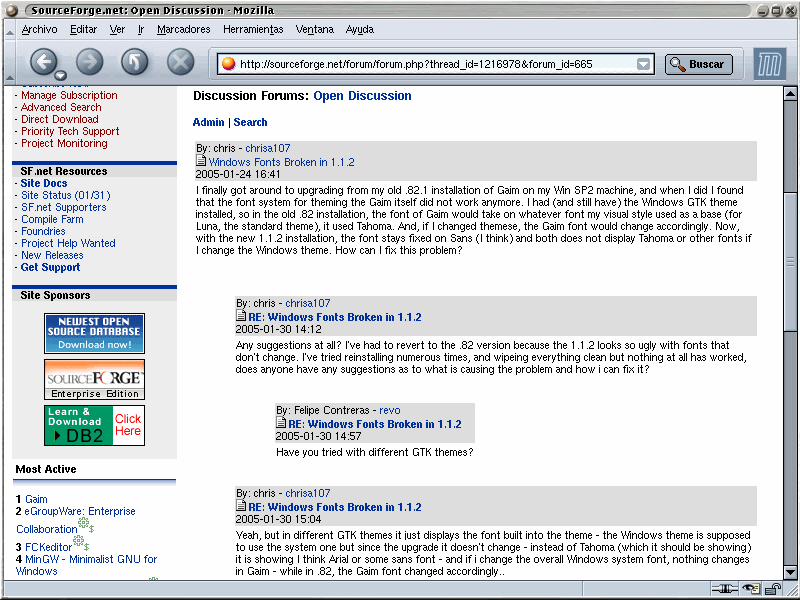
\includegraphics[bb=0 0 800 600, width=12cm, keepaspectratio]{img/foro1}
    \caption{Página con enlaces a hilos}
    \label{figura:foro_hilos}
 \end{figure}

A continuación un bloque ``verbatim'', que se utiliza para mostrar texto tal cual.
Se puede utilizar para ofrecer el contenido de correos electrónicos, código, entre otras cosas.

{\footnotesize
\begin{verbatim}
    From gaurav at gold-solutions.co.uk  Fri Jan 14 14:51:11 2005
    From: gaurav at gold-solutions.co.uk (gaurav_gold)
    Date: Fri Jan 14 19:25:51 2005
    Subject: [Mailman-Users] mailman issues
    Message-ID: <003c01c4fa40$1d99b4c0$94592252@gaurav7klgnyif>
    Dear Sir/Madam,
    How can people reply to the mailing list?  How do i turn off
    this feature? How can i also enable a feature where if someone
    replies the newsletter the email gets deleted?
    Thanks
    From msapiro at value.net  Fri Jan 14 19:48:51 2005
    From: msapiro at value.net (Mark Sapiro)
    Date: Fri Jan 14 19:49:04 2005
    Subject: [Mailman-Users] mailman issues
    In-Reply-To: <003c01c4fa40$1d99b4c0$94592252@gaurav7klgnyif>
    Message-ID: <PC173020050114104851057801b04d55@msapiro>
    gaurav_gold wrote:
    >How can people reply to the mailing list?  How do i turn off
    this feature? How can i also enable a feature where if someone
    replies the newsletter the email gets deleted?
    See the FAQ
    >Mailman FAQ: http://www.python.org/cgi-bin/faqw-mm.py
    article 3.11
\end{verbatim}
}

%%-- Objetivos del  proyecto
%%-- Si la sección anterior ha quedado muy extensa, se puede considerar convertir
%%-- Las siguientes tres secciones en un capítulo independiente de la memoria

\section{Objetivos del proyecto}
\label{sec:objetivos}

\subsection{Objetivo general} % título de subsección (se muestra)
\label{sec:objetivo-general} % identificador de subsección (no se muestra, es para poder referenciarla)


El objetivo de este Trabajo de Fin de Grado es comprobar la capacidad y eficiencia de una Raspberry Pi 4 para entrenar modelos de aprendizaje automático.\\

Aquí vendría el objetivo general en una frase:
Mi Trabajo Fin de Grado/Master consiste en crear de una herramienta de análisis de los comentarios jocosos en repositorios de software libre alojados en la plataforma GitHub.

Recuerda que los objetivos siempre vienen en infinitivo.


\subsection{Objetivos específicos}
\label{sec:objetivos-especificos}

Los objetivos específicos se pueden entender como las tareas en las que se ha desglosado el objetivo general. Y, sí, también vienen en infinitivo.

Lo mejor suele ser utilizar una lista no numerada, como sigue:

    \begin{itemize}
        \item Un objetivo específico.
        \item Otro objetivo específico.
        \item Tercer objetivo específico.
        \item \ldots
    \end{itemize}

\section{Planificación temporal}
\label{sec:planificacion-temporal}

Es conveniente que incluyas una descripción de lo que te ha llevado realizar el trabajo.
Hay gente que añade un diagrama de GANTT.
Lo importante es que quede claro cuánto tiempo has consumido en realizar el TFG/TFM 
(tiempo natural, p.ej., 6 meses) y a qué nivel de esfuerzo (p.ej., principalmente los 
fines de semana).

\section{Estructura de la memoria}
\label{sec:estructura}

Por último, en esta sección se introduce a alto nivel la organización del resto del documento
y qué contenidos se van a encontrar en cada capítulo.

    \begin{itemize}
      \item En el primer capítulo se hace una breve introducción al proyecto, se describen los objetivos del mismo y se refleja la planificación temporal.
      \item En el siguiente capítulo se describen las tecnologías utilizadas en el desarrollo de este TFM/TFG (Capítulo~\ref{chap:tecnologias}).
      \item En el capítulo~\ref{chap:diseño} Se describe el proceso de desarrollo
      de la herramienta \ldots
      \item En el capítulo~\ref{chap:experimentos} Se presentan las principales pruebas realizadas
      para validación de la plataforma/herramienta\ldots (o resultados de los experimentos
      efectuados).
      \item Por último, se presentan las conclusiones del proyecto así como los trabajos futuros que podrían derivarse de éste (Capítulo~\ref{chap:conclusiones}).
    \end{itemize}

\cleardoublepage

%%%%%%%%%%%%%%%%%%%%%%%%%%%%%%%%%%%%%%%%%%%%%%%%%%%%%%%%%%%%%%%%%%%%%%%%%%%%%%%%
%%%%%%%%%%%%%%%%%%%%%%%%%%%%%%%%%%%%%%%%%%%%%%%%%%%%%%%%%%%%%%%%%%%%%%%%%%%%%%%%
% ESTADO DEL ARTE %
%%%%%%%%%%%%%%%%%%%%%%%%%%%%%%%%%%%%%%%%%%%%%%%%%%%%%%%%%%%%%%%%%%%%%%%%%%%%%%%%

\chapter{Estado del arte}               %% a.k.a "Tecnologías utilizadas"
\label{chap:tecnologias}

Descripción de las tecnologías que utilizas en tu trabajo. 
Con dos o tres párrafos por cada tecnología, vale. 
Se supone que aquí viene todo lo que no has hecho tú.

Puedes citar libros, como el de Bonabeau et al., sobre procesos estigmérgicos~\cite{bonabeau:_swarm}. 
Me encantan los procesos estigmérgicos.
Deberías leer más sobre ellos.
Pero quizás no ahora, que tenemos que terminar la memoria para sacarnos por fin el título.
Nota que el \~ \ añade un espacio en blanco, pero no deja que exista un salto de línea. 
Imprescindible ponerlo para las citas.

Citar es importantísimo en textos científico-técnicos. 
Porque no partimos de cero.
Es más, partir de cero es de tontos; lo suyo es aprovecharse de lo ya existente para construir encima y hacer cosas más sofisticadas.
¿Dónde puedo encontrar textos científicos que referenciar?
Un buen sitio es Google Scholar\footnote{\url{http://scholar.google.com}}.
Por ejemplo, si buscas por ``stigmergy libre software'' para encontrar trabajo sobre software libre y el concepto de \emph{estigmergia} (¿te he comentado que me gusta el concepto de estigmergia ya?), encontrarás un artículo que escribí hace tiempo cuyo título es ``Self-organized development in libre software: a model based on the stigmergy concept''.
Si pulsas sobre las comillas dobles (entre la estrella y el ``citado por ...'', justo debajo del extracto del resumen del artículo, te saldrá una ventana emergente con cómo citar.
Abajo a la derecha, aparece un enlace BibTeX.
Púlsalo y encontrarás la referencia en formato BibTeX, tal que así:

\clearpage
{\footnotesize
\begin{minted}{bibtex}
@inproceedings{robles2005self,
  title={Self-organized development in libre software:
         a model based on the stigmergy concept},
  author={Robles, Gregorio and Merelo, Juan Juli\'an 
          and Gonz\'alez-Barahona, Jes\'us M.},
  booktitle={ProSim'05},
  year={2005}
}
\end{minted}
}

Copia el texto en BibTeX y pégalo en el fichero \texttt{memoria.bib}, que es donde están las referencias bibliográficas.
Para incluir la referencia en el texto de la memoria, deberás citarlo, como hemos hecho antes con~\cite{bonabeau:_swarm}, lo que pasa es que en vez de el identificador de la cita anterior (bonabeau:\_swarm), tendrás que poner el nuevo (robles2005self).
Compila el fichero \texttt{memoria.tex} (\texttt{pdflatex memoria.tex}), añade la bibliografía (\texttt{bibtex memoria.aux}) y vuelve a compilar \texttt{memoria.tex} (\texttt{pdflatex memoria.tex})\ldots y \emph{voilà} ¡tenemos una nueva cita~\cite{robles2005self}!

También existe la posibilidad de poner notas al pie de página, por ejemplo, una para indicarte que visite la página del GSyC\footnote{\url{http://gsyc.es}}.

\section{Dispositivo Hardware: Raspberry Pi 4 Modelo B} 
\label{sec:seccion1}

Raspberry Pi es un ordenador de bajo coste y tamaño reducido desarrollado por Raspberry Pi Foundation. Este dispositivo se puede emplear en  multitud de aplicaciones pero su principal objetivo es hacer accesible la informática a todos los usuarios. A parte de poder realizar todas las tareas que se esperan de un ordenador, también puede interactuar con el entorno a través de sensores conectados a sus pines GPIO.

El sistema operativo que ofrece es Raspbian Pi OS, una versión adaptada de Debian. Sin embargo permite utilizar otros sistemas.

Desde su primer lanzamiento se han ido desarrollando y comercializado nuevos modelos. En este proyecto se utilizará la última versión de estos dispositivos denominado como Raspberry Pi 4 Modelo B con 4GB de RAM.

\begin{comment}

\begin{table}
 \begin{center}
  \begin{tabular}{ | l | c | r |} % tenemos tres colummnas, la primera alineada a la izquierda (l), la segunda al centro (c) y la tercera a la derecha (r). El | indica que entre las columnas habrá una línea separadora.
    \hline
    Uno & 2 & 3 \\ \hline % el hline nos da una línea vertical
    Cuatro & 5 & 6 \\ \hline
    Siete & 8 & 9 \\
    \hline
  \end{tabular}
  \caption{Ejemplo de tabla. Aquí viene una pequeña descripción (el \emph{caption}) del contenido de la tabla. Si la tabla no es autoexplicativa, siempre viene bien aclararla aquí.}
  \label{tabla:ejemplo}
 \end{center}
\end{table}
\end{comment}

\section{Gestor de paquetes: Miniforge}
\label{sec:gestor_de_paquetes}

%%-- El comando \gls{} permite incluir términos en el glosario, para luego reunirlos todos
%%-- en una tabla al comienzo o al final del documento, junto con sus definiciones.

Miniforge es un instalador mínimo de conda especifico de conda-forge, que permite instalar el manejador de paquetes conda con una serie de configuraciones predifinidas. Es muy similar a un instalador de Miniconda.

Miniconda es un instalador mínimo de conda, que procede de conda, un sistema de gestión de paquetes y entornos virtuales. Mediante él se instala una pequeña versión de arranque de Anaconda que incluye solo conda, Python, los paquetes de los que dependen y otros pocos paquetes útiles como pueden ser pip, zlib...

Ofrece casi lo mismo que Anaconda pero es mucho más ligero, lo que lo hace idóneo para poder desarrollar el proyecto en el dispositivo utilizado. Además, facilita la replicación de un entorno concreto ya que permite tener un mayor control y orden sobre los paquetes que se instalan. 

\section{Entorno de desarrollo: Jupyter-notebook}
\label{sec:entorno_de_desarrollo}

Jupyter-notebook es una aplicación web de código abierto desarrollada por la organización Proyecto Jupyter. Permite crear y compartir documentos computacionales que siguen un esquema versionado y una lista ordenada de celdas de entrada y de salida. Estas celdas pueden contener código, texto en formato Markdown, fórmulas matemáticas y ecuaciones, o también contenido multimedia. Estas celdas se pueden ejecutar para visualizar los datos y ver los resultados de salida. Además se puede utilizar tanto remotamente como en local.

\section{Lenguaje de programación: Python}
\label{sec:lenguaje_de_programación}

Python es un lenguaje de programación nace a principios de los años 90 gracias al informático holandés Guido Van Rossum. Su objetivo era crear un lenguaje de programación que fuera fácil de aprender, escribir y entender.

Es un lenguaje de alto nivel, interactivo, interpretado y orientado a objetos. Al ser interpretado permite poder ejecutarlo sin necesidad de compilarlo previamente, reduciendo el tiempo entre la escritura y la ejecución del código.
Además es multiplataforma y de código abierto lo que ha ayudado a que Python sea el lenguaje con mayor crecimiento y uno de los más utilizados en la actualidad.  

Entre los campos en los que más se emplea este lenguaje se encuentra la inteligencia artificial, big data, machine learning y data science entre otros, ya que facilita la creación de códigos entendibles de rápido aprendizaje como los que son necesarios en este tipo de proyectos.

\section{Librerías}
\label{sec:Librerías}
Para el desarrollo del proyecto se utilizaron varias librerías que permitiesen la creación de códigos de aprendizaje automático. A continuación se hace mención a las principales y más importantes.

\subsection{Scikit-learn}
\label{subsec:Scikit-learn}
Scikit-Learn es una librería, escrita principalmente en Python, que cuenta con algoritmos de clasificación, regresión, clustering y reducción de dimensionalidad. Fue inicialmente desarrollada por David Cournapeau como proyecto de Google Summer of code en 2007.

La gran variedad de algoritmos y utilidades de Scikit-learn la convierten en la herramienta muy útil para generar aplicaciones de aprendizaje automático.

\subsection{Pandas}
\label{subsec:Pandas}

Pandas es una librería de Python de código abierto, especializada en el manejo y análisis de estructuras de datos. Es muy útil en el ámbito de Data Science y Machine Learning, ya que ofrece unas estructuras muy poderosas y flexibles que facilitan la manipulación y tratamiento de datos.

Tiene todas las funcionalidades necesarias para el análisis de datos como pueden ser: cargar, modelar, analizar, manipular y preparar los datos.

\begin{comment}
PyCharm es un \gls{ide} dedicado concretamente a la programación en Python y desarrollado por la compañía checa JetBrains.

Proporciona análisis de código, un depurador gráfico, una consola de Python integrada, control de versiones y, además, soporta desarrollo web con Django. Todas estas características lo convierten en un entorno completo e intuitivo, idóneo para el desarrollo de proyectos académicos como el que nos ocupa.
\end{comment}

\section{Redacción de la memoria: LaTeX/Overleaf}
\label{sec:redaccion_de_la_memoria}

LaTeX es un sistema de composición tipográfica de alta calidad que incluye características especialmente diseñadas para la producción de documentación técnica y científica. Estas características, entre las que se encuentran la posibilidad de incluir expresiones matemáticas, fragmentos de código, tablas y referencias, junto con el hecho de que se distribuya como software libre, han hecho que LaTeX se convierta en el estándar de facto para la redacción y publicación de artículos académicos, tesis y todo tipo de documentos científico-técnicos. 

Por su parte, Overleaf es un editor LaTeX colaborativo basado en la nube. Lanzado originalmente en 2012, fue creado por dos matemáticos que se inspiraron en su propia experiencia en el ámbito académico para crear una solución satisfactoria para la escritura científica colaborativa.

Además de por su perfil colaborativo, Overleaf destaca porque, pese a que en LaTeX el escritor utiliza texto plano en lugar de texto formateado (como ocurre en otros procesadores de texto como Microsoft Word, LibreOffice Writer y Apple Pages), éste puede visualizar en todo momento y paralelamente el texto formateado que resulta de la escritura del código fuente.

\cleardoublepage

%%%%%%%%%%%%%%%%%%%%%%%%%%%%%%%%%%%%%%%%%%%%%%%%%%%%%%%%%%%%%%%%%%%%%%%%%%%%%%%%
%%%%%%%%%%%%%%%%%%%%%%%%%%%%%%%%%%%%%%%%%%%%%%%%%%%%%%%%%%%%%%%%%%%%%%%%%%%%%%%%
% DISEÑO E IMPLEMENTACIÓN %
%%%%%%%%%%%%%%%%%%%%%%%%%%%%%%%%%%%%%%%%%%%%%%%%%%%%%%%%%%%%%%%%%%%%%%%%%%%%%%%%

\chapter{Diseño e implementación}
\label{chap:diseño}


Aquí viene todo lo que has hecho tú (tecnológicamente). 
Puedes entrar hasta el detalle. 
Es la parte más importante de la memoria, porque describe lo que has hecho tú.
Eso sí, normalmente aconsejo no poner código, sino diagramas.

\section{Configuración del entorno}

Para poder desarrollar correctamente este trabajo es necesario preparar adecuadamente el entorno, una vez acondicionado todo se dará pie al motivo principal de esta investigación.

El primer paso para esto fue montar adecuadamente la Raspberry Pi conforme las instrucciones de Okdo\footnote{\url{https://www.okdo.com/getstarted/}}, empresa de la que procede el kit con el hardware necesario para el proyecto. Una vez está listo el hardware hay que instalar el software necesario para la aplicación de modelos de machine learning.

Empezando por cambiar el sistema operativo, en vez de utilizar el que viene por defecto, Raspbian Pi OS, se instaló Ubuntu 21.10.

Utilizando Miniforge se creo un entorno virtual donde se instalarán todos los paquetes necesarios para el proyecto como son scikit-learn, pandas, jupyter-notebook, stressberry...Estos paquetes permitirán poder desarrollar modelos de aprendizaje automático y poder ponerlos a prueba bajo diferentes estados de la Raspberry.



\section{Arquitectura general} 
\label{sec:arquitectura}

Si tu proyecto es un software, siempre es bueno poner la arquitectura (que es cómo se estructura tu programa a ``vista de pájaro'').

Por ejemplo, puedes verlo en la Figura~\ref{fig:arquitectura}.
\LaTeX \ pone las figuras donde mejor cuadran. 
Y eso quiere decir que quizás no lo haga donde lo hemos puesto\ldots
Eso no es malo.
A veces queda un poco raro, pero es la filosofía de \LaTeX: tú al contenido, que yo me encargo de la maquetación.

\begin{comment}
\begin{figure}
  \centering
  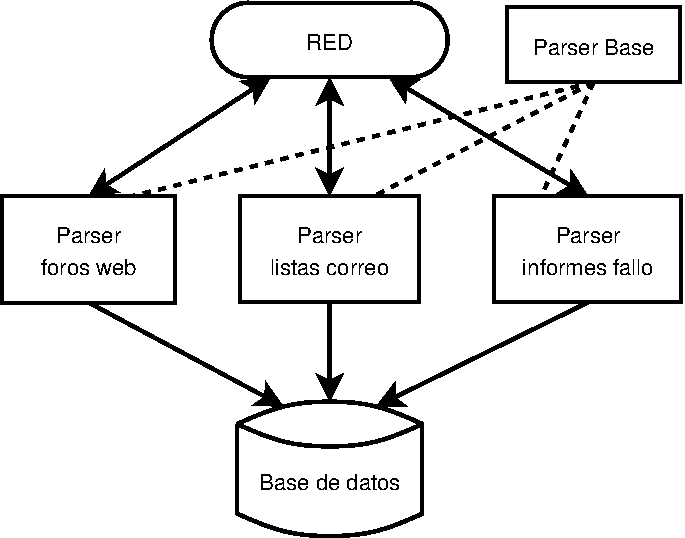
\includegraphics[width=9cm, keepaspectratio]{img/arquitectura.png}
  \caption{Estructura del parser básico.}\label{fig:arquitectura}
\end{figure}

\begin{figure}
    \centering
    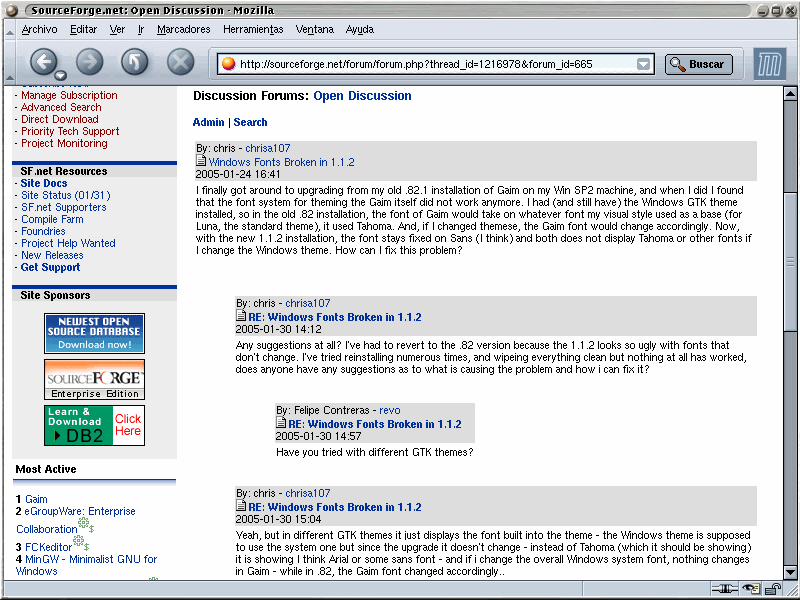
\includegraphics[bb=0 0 800 600, width=12cm, keepaspectratio]{img/foro1}
    \caption{Página con enlaces a hilos}\label{fig:_arquitectura}
\end{figure}
\end{comment}
 
Recuerda que toda figura que añadas a tu memoria debe ser explicada.
Sí, aunque te parezca evidente lo que se ve en la Figura~\ref{fig:arquitectura}, la figura en sí solamente es un apoyo a tu texto.
Así que explica lo que se ve en la Figura, haciendo referencia a la misma tal y como ves aquí.
Por ejemplo: En la Figura~\ref{fig:arquitectura} se puede ver que la estructura del \emph{parser} básico, que consta de seis componentes diferentes: los datos se obtienen de la red, y según el tipo de dato, se pasará a un \emph{parser} específico y bla, bla, bla\ldots

Si utilizas una base de datos, no te olvides de incluir también un diagrama de entidad-relación.

\cleardoublepage

%%%%%%%%%%%%%%%%%%%%%%%%%%%%%%%%%%%%%%%%%%%%%%%%%%%%%%%%%%%%%%%%%%%%%%%%%%%%%%%%
%%%%%%%%%%%%%%%%%%%%%%%%%%%%%%%%%%%%%%%%%%%%%%%%%%%%%%%%%%%%%%%%%%%%%%%%%%%%%%%%
% EXPERIMENTOS Y VALIDACIÓN %
%%%%%%%%%%%%%%%%%%%%%%%%%%%%%%%%%%%%%%%%%%%%%%%%%%%%%%%%%%%%%%%%%%%%%%%%%%%%%%%%

\chapter{Experimentos y validación}
\label{chap:experimentos}

\textbf{Atención}: Este capítulo se introdujo como requisito en 2019.

\begin{comment}
Describe los experimentos y casos de test que tuviste que implementar para validar tus resultados. 
Incluye también los resultados de validación que permiten afirmar que tus resultados son correctos.
\end{comment}

La primera prueba realizada para observar el comportamiento de la Raspberry para generar un modelo de aprendizaje automático, fue intentar generar mediante scripts de Python tres diferentes modelos de aprendizaje supervisado para realizar una clasificación binaria, basados en regresión logística, máquinas de soporte vectorial y gradient tree boosting.

Para ello se utilizó el data set de Room Occupancy detection data, obtenido de Kaggle\cite{DataSetOccuapncy}, que contiene unas 20560 muestras. Cada ejemplo tiene las medidas de temperatura, humedad, CO2 y luz de una habitación de oficina de unos quince metros cuadrados. La última columna de cada fila indica la clase a la que pertenece la muestra. En este caso, al ser una clasificación binaria esta última columna solo puede tener dos valores, cero o uno. Si para un ejemplo contiene un uno significa que para esos valores sensados la habitación está ocupada. Si por el contrario hay un valor de cero la sala está vacia. 

Para generar los modelos se dividió el set de datos en dos partes, una primera parte para entrenar (que contenía el 70\% de ejemplos del set de datos original) y otra para comprobar la eficiencia del modelo a la hora de clasificar si la estancia está ocupada o no. En esta segunda parte se utilizó el 30\% restante de muestras del set de datos original, que no se utilizaban en el entrenamiento y por lo tanto el modelo nunca los ha visto, son totalmente nuevos para el. Un aspecto importante a destacar de este set de datos es que hay una mayor cantidad de ejemplos de habitación no ocupada que de ocupada. En otros sets de datos esto podría representar un problema ya que puede dar lugar a que al realizar esta división de forma aleatoria, el conjunto de datos de entrenamiento apenas tenga ejemplos de una de las clases. Sin embargo al tener una gran número de ejemplos en el que ambas clases tienen una gran cantidad de muestras, como es este caso, una división aleatoria no representa ningún inconveniente dado que hay una alta probabilidad de que el set de entrenamiento siempre tenga como mínimo la cantidad de muestras necesarias de ambas clases para entrenar correctamente. Aun así, la división se realizó de forma estratificada, para que hubiese la misma proporcion de datos de una clase u otra que en el set de datos original. Y de esta forma nos aseguramos que a la hora de tanto entrenar, como de comprobar el modelo generado, se tenga ejemplos de ambas clases en la misma proporción que aparecen en el set de datos original.

Con esta división y preparación de los datos, los tres modelos se pudieron generar sin problemas utilizando las librerías de scikit-learn y pandas. Todos conseguían una accuracy superior al 90\%, el tiempo de ejecución era de unos cinco segundos salvo para gradient tree boosting, que tardaba unos siete segundos.

Dado que no hubo ningún tipo de problema con la ejecución de los scripts, se procedió a realizar los mismos modelos pero utilizando esta vez Jupyter-notebook. Con esto la Raspberry pudo seguir ejecutando los algoritmos sin problemas. 

Se añadió un poco más de dificultad a la Raspberry haciendo que los algoritmos utilizasen validación cruzada, es decir, que dentro del set de datos de entrenamiento (compuesto, una vez más, por el 70\% de ejemplos del set de datos original) se hace una subdivisión en otros cinco sets para entrenar y probar el modelo con cada uno de ellos. Una vez realizada la validación cruzada se vuelve a probar la eficiencia del modelo haciendo que clasifique el 30\% de datos de la división original, son datos que nunca ha visto ni entrenado con ellos. El objetivo de realizar una validacion cruzada es poder obtener una estimación más realista en base a las estimaciones de los experimentos individuales, que rotan los datos usados para entrenar. Los resultados de esta prueba siguieron siendo muy buenos (el acierto seguía estando por encima del 90\%). Y mientras que en el modelo de regresión logística el tiempo de ejecución se mantuvo más o menos igual, en el caso de las máquinas de soporte vectorial y gradient tree boosting los tiempos de ejecución aumentaron. Con SVM la ejecución llega a los siete segundos de media, y para gradient tree boosting a unos dieciseis segundos.
 
\section{Incorporación de código en la memoria}

Es bastante habitual que se reproduzcan fragmentos de código en la memoria de un TFG/TFM.
Esto permite explicar detalladamente partes del desarrollo que se ha realizado que se consideren
de especial interés. No obstante, tampoco es conveniente pasarse e incluir demasiado código en
la memoria, puesto que se puede alargar mucho el documento. Un recurso muy habitual es subir
todo el código a un repositorio de un servicio de control de versiones como GitHub o GitLab,
y luego incluir en la memoria la URL que enlace a dicho repositorio.

Para incluir fragmentos de código en un documento \LaTeX se pueden combinar varias
herramientas:

\begin{itemize}
    \item El entorno \mintinline{latex}{\begin{listing}[]...\end{listing}} permite crear
    un marco en el que situar el fragmento de código (parecido al generado cuando insertamos
    una tabla o una figura). Podemos insertar también una descripción (\textit{caption})
    y una etiqueta para referenciarlo luego en el texto.
    
    \item Dentro de este entorno, se puede utilizar el paquete 
    \mintinline{latex}{minted}~\footnote{\url{https://es.overleaf.com/learn/latex/Code_Highlighting_with_minted}},
    que utiliza el paquete Python Pygments para resaltado de sintaxis (coloreando el
    código). Como se puede ver en el siguiente ejemplo, hay muchas opciones de configuración
    que permiten controlar cómo se va a mostrar el código (incluir números de línea, saltos
    de línea, tamaño y tipo de fuente, espaciado, código de colores para resaltado, etc.).
\end{itemize}

\begin{listing}[h!]
    \caption{Lectura de un fichero *.csv y tipado de datos.}{}
    \label{lst:1}
    \begin{minted}[breaklines, fontsize=\footnotesize, baselinestretch=1]{python}
# A dictionary is built to define the data type contained by each column
dtype_scheme ={'budget': np.int64, 'genres': np.object, 'homepage': np.str, 'id': np.int64, 'keywords': np.object, 'original_language': np.str, 'original_title': np.str, 'overview': np.str, 'popularity': np.float64, 'production_companies': np.object, 'production_countries': np.object, 'release_date': np.object, 'revenue': np.int64, 'runtime': np.float64, 'spoken_languages': np.object,  'status': np.object, 'tagline': np.str, 'title': np.str, 'vote_average': np.float64, 'vote_count': np.int64}

# When loading the data from the .csv file, we provide the scheme to be followed for data typing
df1 = dd.read_csv('tmdb_5000_movies.csv', dtype=dtype_scheme)
    \end{minted}
\end{listing}

Otra ventaja del entorno \verb|listing| es que se puede generar automáticamente un índice
(con entradas hiperenlazadas) de fragmentos de código, para incluirlo al comienzo del 
documento junto con los índices de figuras, tablas, etc.

\subsection{Fuentes monoespaciadas}

A veces se incluyen nombres de archivos, paquetes, etc. como texto monoespaciado, utilizando
el comando \LaTeX \mintinline{latex}{\texttt{}}. Sin embargo, esto puede generar un problema
cuando las palabras en fuente monoespaciada alcanzan el final de una línea. En ese caso,
el compilador rehusa muchas veces romper la palabra y deja la línea demasiado larga respecto
al resto.

Para evitar esto, especialmente en párrafos más cortos de lo habitual (como en una lista
no numerada), se puede utilizar el comando \mintinline{latex}{\begin{sloppypar}...\end{sloppypar}},
como se muestra a continuación con un ejemplo real.
    
\begin{itemize}
    
    \begin{sloppypar} % Arregla longitud de línea en párrafos con fuente monoespaciada
    \item Los valores contenidos en las columnas \texttt{genres}, \texttt{spoken\_languages}, \texttt{production\_companies} y \texttt{production\_countries}, clasificados originalmente como \texttt{np.objects}, se corresponden en realidad con listas de objetos \gls{json} que han sido almacenadas como cadenas de caracteres. A través de la función \texttt{get\_values(obj, key)} definida específicamente para ello, se transformará dicha cadena de caracteres en una lista de diccionarios a través de la función \texttt{json.loads(obj)} y se devolverá una  tupla que recopile los valores de los mismos para la clave indicada, un objeto de Python mucho más manejable de cara a realizar consultas sobre el \textit{dataset}.
    \end{sloppypar}
    
\end{itemize}

\cleardoublepage

%%%%%%%%%%%%%%%%%%%%%%%%%%%%%%%%%%%%%%%%%%%%%%%%%%%%%%%%%%%%%%%%%%%%%%%%%%%%%%%%
%%%%%%%%%%%%%%%%%%%%%%%%%%%%%%%%%%%%%%%%%%%%%%%%%%%%%%%%%%%%%%%%%%%%%%%%%%%%%%%%
% CONCLUSIONES %
%%%%%%%%%%%%%%%%%%%%%%%%%%%%%%%%%%%%%%%%%%%%%%%%%%%%%%%%%%%%%%%%%%%%%%%%%%%%%%%%


\chapter{Conclusiones y trabajos futuros}
\label{chap:conclusiones}


\section{Consecución de objetivos}
\label{sec:consecucion-objetivos}

Esta sección es la sección espejo de las dos primeras del capítulo de objetivos, donde se planteaba el objetivo general y se elaboraban los específicos.

Es aquí donde hay que debatir qué se ha conseguido y qué no. 
Cuando algo no se ha conseguido, se ha de justificar, en términos de qué problemas se han encontrado y qué medidas se han tomado para mitigar esos problemas.

Y si has llegado hasta aquí, siempre es bueno pasarle el corrector ortográfico, que las erratas quedan fatal en la memoria final.
Para eso, en Linux tenemos aspell, que se ejecuta de la siguiente manera desde la línea de \emph{shell}:

\begin{minted}{bash}
  aspell --lang=es_ES -c memoria.tex
\end{minted}

\section{Aplicación de lo aprendido}
\label{sec:aplicacion}

Aquí viene lo que has aprendido durante el Grado/Máster y que has aplicado en el TFG/TFM. Una buena idea es poner las asignaturas más relacionadas y comentar en un párrafo los conocimientos y habilidades puestos en práctica.

\begin{enumerate}
  \item a
  \item b
\end{enumerate}


\section{Lecciones aprendidas}
\label{sec:lecciones_aprendidas}

Aquí viene lo que has aprendido en el Trabajo Fin de Grado/Máster.

\begin{enumerate}
  \item Aquí viene uno.
  \item Aquí viene otro.
\end{enumerate}


\section{Trabajos futuros}
\label{sec:trabajos_futuros}

Ningún proyecto ni software se termina, así que aquí vienen ideas y funcionalidades que estaría bien tener implementadas en el futuro.

Es un apartado que sirve para dar ideas de cara a futuros TFGs/TFMs.

\chapter{Anexo}
\label{chap:anexo}

En la preparación del entorno para el desarrollo de este proyecto surgieron algunas dificultades.\\
Como se comenta en el capítulo 3 uno de los primeros pasos fue instalar Miniforge, pero antes de instalar este gestor de paquetes se intentó utilizar Miniconda en el sistema operativo que viene por defecto en la Raspberry (Raspbian Pi OS), de forma que permitiese crear un entorno virtual con una versión de Python superior a la 3.7. Sin embargo, debido a la arquitectura de 32-bit empleada por dicho sistema operativo, no era posible instalar una versión de Python superior a la 3.6 por medio de Miniconda, pues para esas versiones se requería una arquitectura de 64-bit.

Por lo que fue necesario instalar Ubuntu 21.10 cuya arquitectura es de 64-bit. Aún así, tampoco se pudo instalar Miniconda con una versión de Python 3.8 o 3.9. La solución recayó en instalar Miniforge que proporciona un administrador de paquetes conda, muy similar a la función que desempeña Miniconda.

Una vez creado el entorno virtual con una verisón de Python igual a la 3.9, se procedió a intentar acceder a los pines GPIO desde este mismo entorno. Para poder acceder a ellos comunmente siempre se ha utilizado un paquete denominado RPi.GPIO, pero los métodos utilizados por dicho paquete para la comunicación con los pines de la Raspberry dejaron de funcionar en versiones de kernels de Linux iguales o superiores a la 5.11. La versión de kernel utilizada en este trabajo es la 5.13, por tanto la librería GPIO no puede resolver la comunicación con los pines.

Para versiones de Ubuntu iguales o superiores a la 21.04, existe un nuevo paquete llamado LGPIO que implementa las funciones necesarias para poder acceder a los pines. Para poder utilizar este paquete dentro del entorno virtual creado, fue necesario instalarlo primeramente fuera de este, utilizando sudo apt-get install para después mover manualmente los ficheros instalados dentro del directorio del entorno virtual. Con esto, y ejecutando el fichero con permisos de root, finalmente se puede acceder a los pines y por lo tanto leer o escribir en ellos.\\
Cuando se quiere instalar un paquete dentro del entorno se utilizan los comandos conda install o bien pip3 install, sin embargo, por ninguno de estos dos medios se pudo obtener LGPIO de forma funcional.

También dentro del entorno creado se instaló todo lo necesario para realizar este proyecto. Entre estos paquetes se instaló la librería de scikit-learn que tiene algoritmos para generar modelos de clasificación, regresión, clustering y reducción de la dimensionalidad. Así como pandas que tiene todas las funcionalidades necesarias para el análisis de datos como pueden ser: cargar, modelar, analizar, manipular y preparar los datos.

Además se instaló stressberry que es un paquete para hacer pruebas de temperatura bajo diferentes cargas computacionales mostrando los resultados obtenidos por medio de plots. En este caso, dicho paquete se utilizará para poder someter a la Raspberry a diferentes niveles de estrés y de este modo ver su capacidad para entrenar modelos de aprendizaje automático. Para poder ejecutar stressberry hay que tener en cuenta que el usuario que ejecute este comando debe pertenecer al grupo video, de lo contrario la ejecución dará error.

A parte de poder comprobar la capacidad de la Raspberry para ejecutar estos programas bajo diferentes cargas computacionales, también permitirá comparar los tiempos de ejecución con respecto a los tiempos que alcanzan dichos programas en un portátil corriente.

%%%%%%%%%%%%%%%%%%%%%%%%%%%%%%%%%%%%%%%%%%%%%%%%%%%%%%%%%%%%%%%%%%%%%%%%%%%%%%%%
%%%%%%%%%%%%%%%%%%%%%%%%%%%%%%%%%%%%%%%%%%%%%%%%%%%%%%%%%%%%%%%%%%%%%%%%%%%%%%%%
% GLOSARIO(S) %
%%%%%%%%%%%%%%%%%%%%%%%%%%%%%%%%%%%%%%%%%%%%%%%%%%%%%%%%%%%%%%%%%%%%%%%%%%%%%%%%

\printglossary[type=\acronymtype]

\printglossary

%%%%%%%%%%%%%%%%%%%%%%%%%%%%%%%%%%%%%%%%%%%%%%%%%%%%%%%%%%%%%%%%%%%%%%%%%%%%%%%%
%%%%%%%%%%%%%%%%%%%%%%%%%%%%%%%%%%%%%%%%%%%%%%%%%%%%%%%%%%%%%%%%%%%%%%%%%%%%%%%%
% APÉNDICE(S) %
%%%%%%%%%%%%%%%%%%%%%%%%%%%%%%%%%%%%%%%%%%%%%%%%%%%%%%%%%%%%%%%%%%%%%%%%%%%%%%%%

%\cleardoublepage
%\appendix
%\chapter{Manual de usuario}
%\label{app:manual}


%%%%%%%%%%%%%%%%%%%%%%%%%%%%%%%%%%%%%%%%%%%%%%%%%%%%%%%%%%%%%%%%%%%%%%%%%%%%%%%%
%%%%%%%%%%%%%%%%%%%%%%%%%%%%%%%%%%%%%%%%%%%%%%%%%%%%%%%%%%%%%%%%%%%%%%%%%%%%%%%%
% BIBLIOGRAFIA %
%%%%%%%%%%%%%%%%%%%%%%%%%%%%%%%%%%%%%%%%%%%%%%%%%%%%%%%%%%%%%%%%%%%%%%%%%%%%%%%%

\cleardoublepage

%% OLD BIBTEX CODE, TO BE DELETED
%\bibliographystyle{abbrv}
%\bibliographystyle{plain} 
%\bibliography{memoria}  % memoria.bib es el nombre del fichero que contiene las referencias bibliográficas.

% https://www.overleaf.com/learn/latex/Bibliography_management_with_biblatex
\raggedright\printbibliography[heading=bibintoc,title={Referencias}]

\end{document}
